%%=============================================================================
%% Discussie
%%=============================================================================

\chapter{\IfLanguageName{dutch}{Discussie}{Discussion}}%
\label{ch:discussie}

In dit hoofdstuk worden de resultaten uit de requirementsanalyse, vergelijkende studie en de ontwikkeling van het prototype besproken. 

\section{Requirementsanalyse}

% Startende zin over lexicale vereenvoudiging
Woorden- en synoniemenlijsten kunnen een ondersteunend middel aanbieden voor zowel scholieren met dyslexie als zonder bij het lezen van wetenschappelijke artikelen en wordt aangeboden in Kurzweil. Automatisch genereren is enkel prevalent binnen ChatGPT en de Bing chatbot, maar de tools houden geen rekening met de doelgroep, tenzij expliciet aangegeven met een one-shot summary. Andere tools houden helemaal geen rekening met de doelgroep en kunnen enkel woordenlijsten genereren op basis van gekozen woorden. 

\medspace


Bij de geteste tools is PDF-upload de standaardmethode. Het inlezen van tekstinhoud is beschikbaar bij de webtoepassingen, maar niet bij de erkende software in het onderwijs. ChatGPT en Bing chatbot genereren mensachtige teksten, maar kunnen geen PDF's verwerken. Het kopiëren en plakken van tekst uit het originele document kan leiden tot weinig fouten, maar is omslachtig en moet verbeterd worden. Bestaande tools hebben moeite met oudere PDF's waarbij niet alle tekst kan worden geëxtraheerd. Een geavanceerde optie voor het inlezen van PDF's is vereist.

\medspace

Tools spenderen weinig tijd op de analyse over het ingegeven document, alsook het vereenvoudigde of samengevatte document. Simplish doet dit wel en geeft aan de hand van kleurcodes bepaalde data over de vereenvoudigde tekst mee, waaronder niet-veranderende woorden, adequate vertalingen, uitleg naar de voetnoot, homoniemen of woorden waarvan er geen eenvoudig synoniem is. Zoals aangegeven in \ref{img:simplish-output} duidt de vergelijkende weergave de verschillen aan tussen de oorspronkelijke en vereenvoudigde tekst en met behulp van kleurcodes worden de verschillende transformaties aangegeven.

\begin{figure}[H]
	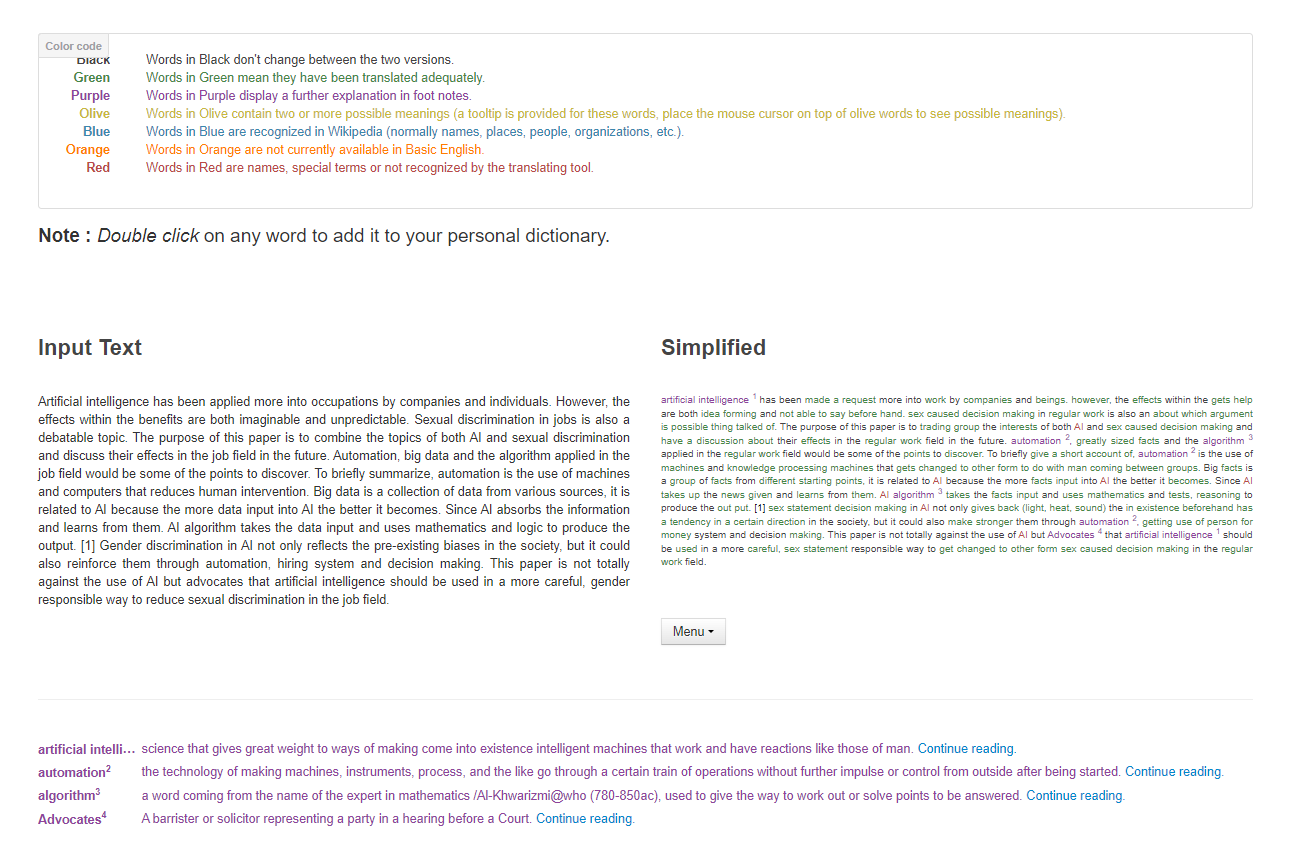
\includegraphics[width=\linewidth]{img/simplish-output.png}
	\label{img:simplish-output}
\end{figure}

\begin{center}
	\begin{tabular}{ | m{4cm} | m{12cm} | } 
		\hline
		\textbf{MoSCoW-principe} & Functionaliteit \\
		\hline
		Must-have & Gepersonaliseerde vereenvoudiging aanbieden, waaronder lexicale en syntactische vereenvoudiging aanbieden, na het toevoegen van een respectievelijke API-sleutel. \\
		& Wetenschappelijke artikelen in PDF-vorm opladen. \\
		& Personaliseerbare site: lettertype -en grootte aanpassen, tekstformaat aanpassen, achtergrondkleur aanpassen \\
		& Lokale opzet \\
		\hline
		Should-have & Glossary genereren na handmatige selectie van moeilijke woorden \\
		& Personaliseerbare PDF- of Worddocumentlay-out \\
		& Uitvoer als PDF of Word-bestand teruggeven. \\
		\hline
		Could-have & Glossary genereren na automatische selectie van moeilijke woorden \\
		\hline
		Wont-have & Beschikbaarheid tot de tool zonder Docker Desktop, in de vorm van online webtoepassing of browserextensie. \\
		& Beschikbaarheid tot de standaard- en gepersonaliseerde opties zonder API-sleutels \\
		\hline
	\end{tabular}
\end{center}

\section{Vergelijkende studie}

De huidige softwaretools die worden gebruikt in het middelbaar onderwijs zijn niet in staat om de oorspronkelijke tekst te transformeren, wat betekent dat syntactische vereenvoudiging momenteel niet haalbaar is. Hoewel er online webtoepassingen beschikbaar zijn, bieden ze minder functionaliteiten om de moeilijkheidsgraad van zinsyntaxis te verlagen en zijn ze voornamelijk gericht op het verkorten van de oorspronkelijke tekst ofwel samenvatting. Het aanpassen van tangconstructies, verwijswoorden, voorzetseluitdrukkingen, samengestelde werkwoorden en onregelmatige werkwoorden blijft daarom een uitdaging voor deze toepassingen. Zelfs het schrijven in de actieve stem kan problematisch zijn, en er zijn alleen vooraf gedefinieerde prompts beschikbaar om deze transformaties uit te voeren.

\medspace

Hoewel taalmodellen zoals GPT-3 in staat zijn om zinsyntaxtransformaties uit te voeren, kunnen ze soms problemen ondervinden bij het verwerken van alle meegegeven transformaties, en er is geen garantie dat deze modellen alle transformaties met slechts één prompt kunnen uitvoeren. Om deze uitdagingen aan te pakken, kunnen bestaande pipelines voor tekstvereenvoudiging gebruikmaken van verschillende transformers, waarbij de tekst meerdere keren aan het GPT-3 model wordt gegeven maar met verschillende prompts. Het moet echter opgemerkt worden dat taalmodellen van HuggingFace minder gericht zijn op het aanpassen van de zinsyntaxis en vaak vrijwel identieke tekst genereren.

\medspace

\subsection{Conclusie}

Ontwikkelaars kunnen voor algemene samenvattings- en vereenvoudigingstaken gebruik maken van algemene taalmodellen die vrij beschikbaar op \textit{HuggingFace} of dergelijke platforms terug te vinden zijn. GPT-3 blinkt uit in gepersonaliseerde vereenvoudigings- en samenvattingstaken. Engelstalige prompts die expliciet de uitvoertaal vermelden zijn nauwkeuriger dan Nederlandstalige prompts. 

\section{Opbouw van het prototype}

Deze ontwerpkeuze bespaart geheugenruimte voor ontwikkelaars en vermindert de benodigde rekenkracht voor een prototype. Eenmaal ontwikkelaars de toepassing willen uitrollen naar het grote publiek, wordt er net zoals bij (...) aangeraden om de taalmodellen zelf te hosten.
